\chapter{Resultados y conclusiones}\label{chap:part1conclusions}

Para poder valorar la utilidad real del sistema de medida que se ha
desarrollado en este proyecto frente a las distintas alternativas que
existen, dispositivos que realizan una función semejante, se ha decidido
comparar los resultados que se obtienen al utilizar este sistema y los que
se obtienen al utilizar un osciloscopio (como elemento representativo del
conjunto de alternativas al sistema) en una prueba genérica.

Por separado se ha evaluado el rendimiento del subsistema de interacción
con el medio físico (el conjunto formado por los circuitos acondicionadores
y los transductores de ultrasonidos).


\section{Objetivos}

El objetivo de la prueba de rendimiento es determinar las prestaciones y
limitaciones del sistema de medida desarrollado. Para ello se han comparado
los resultados obtenidos al visualizar una batería de señales en un
osciloscopio de laboratorio y en el sistema de medida. Los parámetros que
se han evaluado son los siguientes.

\begin{itemize}
    \item Medida en tiempo real de la amplitud de la señal en ambos
	dispositivos.
    \item Medida en tiempo real de la frecuencia de la onda eléctrica.
    \item Fidelidad de la representación.
    \item Capacidad para seguir la forma de la onda en el modo continuo de
	representación.
\end{itemize}

Se ha realizado además una prueba secundaria para poder determinar que las
funciones de la aplicación de control operan satisfactoriamente.


\section{Metodología}\label{sec:working-test}

El procedimiento de medida consta de unos sencillos pasos. Previamente a la
realización de las observaciones se dispone el equipo. El equipo utilizado
está formado por los siguientes elementos:

\begin{itemize}
    \item Generador de señales, utilizado para generar la distintas señales
	utilizadas para las pruebas.
    \item Osciloscopio, en el que se observa la representación que sirve de
	referencia para la comparación.
    \item Un equipo (\pc{}) en el que se encuentran previamente instaladas
	la tarjeta de adquisición y la aplicación de control.
    \item La caja de conexiones desarrollada para la tarjeta de
	adquisición (\vref{fig:conbox}).
    \item Sondas terminadas en ambos extremos con conectores de tipo banana
	compatibles con la caja de conexiones.
    \item Sondas para el osciloscopio y el generador de señales.
\end{itemize}

Los pasos seguidos para evaluar la bondad de la representación de la señal
que realiza el sistema de medida se enumeran a continuación.

\begin{enumerate}
    \item Se lanza la aplicación de control.
    \item Se configura el osciloscopio para que proporcione una medida de
	la amplitud de la señal en Vpp y de su frecuencia.
    \item Se selecciona una forma de onda en el generador de señales.
    \item Para la onda seleccionada se elige una amplitud de 16 Vpp.
    \item Se selecciona una frecuencia del conjunto expuesto en el
	\cref{tab:testparameters} empezando por la frecuencia más baja del
	rango.
    \item Se observa la señal representada en el osciloscopio y en el
	sistema de medida, comparando si la segunda es fiel a la primera.
	Se anotan los valores observados de amplitud y frecuencia en ambos
	dispositivos.
    \item Se repiten los pasos desde el paso 5 hasta agotar todas las
	frecuencias. Después se selecciona una frecuencia fija de 1 kHz y
	se repite el procedimiento para distintos valores de amplitud.
    \item Se repite todo el procedimiento desde el tercer paso hasta haber
	completado la prueba para todos los tipos de señal evaluados.
\end{enumerate}

Cabe mencionar que mientras que el osciloscopio proporciona automáticamente
un valor de frecuencia y uno de amplitud para cada señal evaluada, en el
sistema de medida es preciso determinar esos valores a partir de la señal
representada (amplitud) y su espectro en frecuencias (frecuencia central).

El \cref{tab:testparameters} muestra los parámetros de la prueba: los
distintos tipos de señal evaluados; los valores de frecuencia y los valores
de amplitud.

\begin{table}
    \centering
    \begin{tabular}{l d{5.1}d{8.1}d{2.1}}
	\toprule
	& \multicolumn{3}{c}{Parámetros de la señal} \\
	\cmidrule(l){2-4}
	Tipo de señal & \multicolumn{1}{c}{Frecuencia (Hz)} &
	    \multicolumn{1}{c}{Periodo ($\mu\text{s}$)} &
	    \multicolumn{1}{c}{Amplitud (Vpp)} \\
	\midrule
		    & 0,1	& 10000000	& \\
		    & 1		& 1000000	& \\
	Sinusoidal  & 5		& 200000	& 16 \\
		    & 25	& 40000		& \\
	Rectangular & 100	& 10000		& 10 \\
		    & 1000	& 1000		& \\
	Triangular  & 10000	& 100		& 1 \\
		    & 20000	& 50		& \\
	Pulsada	    & 30000	& 33,3		& 0,1 \\
		    & 40000	& 25		& \\
		    & 50000	& 20		& \\
	\bottomrule
    \end{tabular}
    \caption[Parámetros de la prueba]{Parámetros de la prueba.}
    \label{tab:testparameters}
\end{table}


\subsection{Procedimiento, prueba secundaria}

El objetivo de la prueba secundaria es el de establecer que las distintas
funciones implementadas en la aplicación de control realizan su cometido
satisfactoriamente. Para la realización de esta prueba se ha empleado el
mismo equipo que en la prueba principal. El procedimiento que se ha seguido
consta de una serie de pasos que se enumeran a continuación.

\begin{enumerate}
    \item Tras disponer el equipo y conectar los dispositivos se ajusta el
	generador de señales para que transmita una onda sinusoidal de 1~Hz
	de frecuencia y una amplitud de 1 Vpp.
    \item Se comprueba que las medidas numéricas se correspondan con lo
	esperado.
    \item Después se ajusta la frecuencia de muestreo y la ganancia del
	amplificador interno de la tarjeta de adquisición y se comparan los
	resultados.
    \item La sonda que transmite la señal al sistema de medida se conecta a
	cada puerto de entrada y se evalúa que estos funcionan
	correctamente. Para ello se selecciona cada vez el canal adecuado
	en la aplicación de control.
    \item Se ajusta el generador de señales para que transmita esta vez una
	señal de 4 kHz y 16 Vpp.
    \item Se evalúan las distintas opciones del modo gráfico de
	funcionamiento: selección de la escala temporal, selección de la
	escala de amplitud, selección del número de puntos para la
	realización de la \sig{fft}, representación de la señal y su
	espectro en frecuencias en la ventana de representación elegida,
	habilitación o inhabilitación de alguna o ambas representaciones.
\end{enumerate}


\section{Resultados}

Dada la multitud de variables que intervienen en la realización de las
pruebas se obtiene una gran cantidad de resultados, en este documento se ha
optado por ofrecer sólo una muestra representativa de los mismos
(\cref{tab:measureresults}).

\begin{table}
    \centering
    \begin{tabular}{ld{2,1}d{2,4}}
	\toprule
	& \multicolumn{2}{c}{Valores en el sistema} \\
	\cmidrule(r){2-3}
	Señal evaluada & \multicolumn{1}{c}{amplitud (Vpp)} &
	    \multicolumn{1}{c}{frecuencia (kHz)} \\
	\midrule
	sinusoidal @ 16 Vpp, 1 Hz & 16 & \sim0,001 \\
	sinusoidal @ 16 Vpp, 5 Hz & 16 & 0,005 \\
	sinusoidal @ 0,1 Vpp, 10 kHz & 0,1 & 9,9 \\
	sinusoidal @ 16 Vpp, 10 kHz & 16 & 10 \\
	rectangular @ 16 Vpp, 10 kHz & 16 & 9,5 \\
	triangular @ 16 Vpp, 10 kHz & 15,4 & 9,35 \\
	pulsada @ 16 Vpp, 10 kHz & \text{---} & \text{---} \\
	sinusoidal @ 16 Vpp, 20 kHz & 16 & 20 \\
	sinusoidal @ 16 Vpp, 40 kHz & 16 & 40 \\
    \end{tabular}
    \caption[Resultados obtenidos]{Resultados obtenidos, se ha omitido la
    columna correspondiente al osciloscopio.}
    \label{tab:measureresults}
\end{table}


\subsubsection{Observaciones}

Complementando los resultados expuestos en el \cref{tab:measureresults} se
hacen las siguientes observaciones sobre la fidelidad de la representación
de la señal que se observa en la interfaz del software de control.

A frecuencias por debajo de 1 Hz el disparo del sistema empieza a fallar
(del mismo modo que ocurre en los osciloscopios), por lo que se hace
necesario representar la señal en modo continuo. Se ha observado que en
sistemas con un rendimiento gráfico bajo la representación vista en el
sistema de medida cuando representa en modo continuo no consigue seguir a
la señal, pueden verse escalones correspondientes al instante en el que el
búffer de la aplicación se refresca.

Por otro lado, al ser limitada la frecuencia de muestreo del dispositivo de
adquisición, la representación de la señal empieza a perder forma (aunque
se siguen observando valores correctos de amplitud y frecuencia) a partir
de los 25 kHz aproximadamente.

Por último se ha advertido que la caja de conexiones presenta un fallo.
Cuando se inserta señal a través de un puerto analógico parte de esa señal
se observa en el resto de puertos de la misma fila (existen dos filas de
puertos, una del 0 al 7 y otra del 8 al 15). Ello impide que se puedan
utilizar dos puertos de la tarjeta simultáneamente (ha de recalcarse que se
trata de un fallo en la caja de conexiones y no en la aplicación de
control).


\subsection{Resultados, prueba secundaria}

Las pruebas realizadas determinan que la aplicación de control no está
afectada por ningún defecto de funcionamiento excepto por los observados en
este apartado.

Las imágenes expuestas a continuación en las
\crefrange{fig:default}{fig:point-number} muestran que los controles que
regulan el comportamiento del modo gráfico de funcionamiento realizan su
función satisfactoriamente. Sin embargo se observa un fallo de
funcionamiento probablemente debido al equipo en el que se han desarrollado
las pruebas: en ocasiones al lanzar la aplicación \matlab{} deja de
responder y el controlador de la tarjeta queda bloqueado, cuando esto
ocurre es necesario reiniciar el equipo para poder volver a utilizar el
sistema.

\begin{figure}
    \begin{center}
	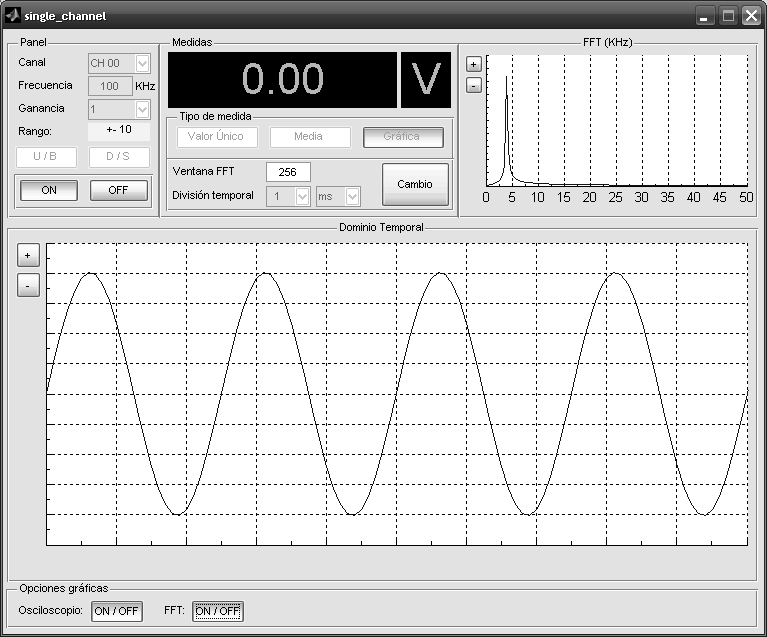
\includegraphics{gis-pfc-ch4-01.png}
    \end{center}
    \caption[Configuración por defecto]{Representación de los datos
    utilizando la configuración por defecto.}
    \label{fig:default}
\end{figure}

\begin{figure}[p]
    \begin{center}
	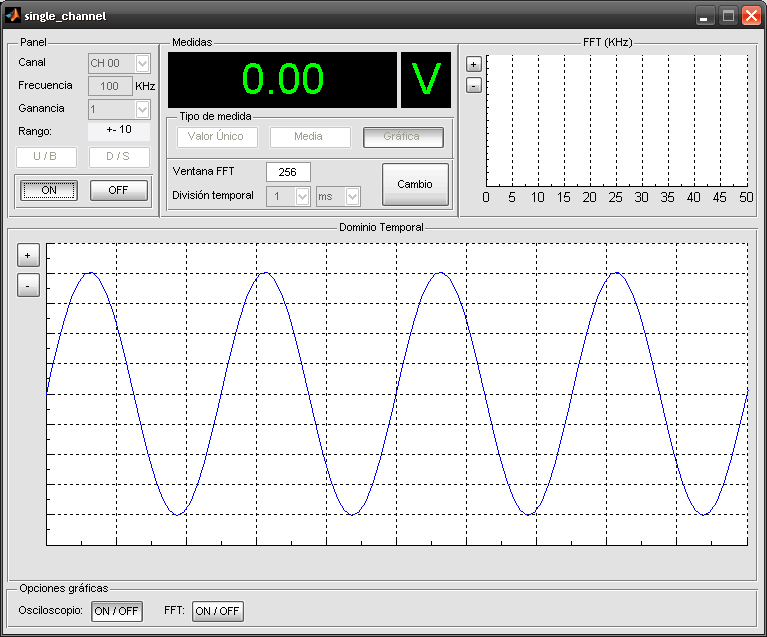
\includegraphics{gis-pfc-ch4-02.png}
    \end{center}
    \caption[Representación del espectro de la señal
    inhabilitada]{Representación del espectro de la señal inhabilitada.}
    \label{fig:specter-disabled}
\end{figure}

\begin{figure}[p]
    \begin{center}
	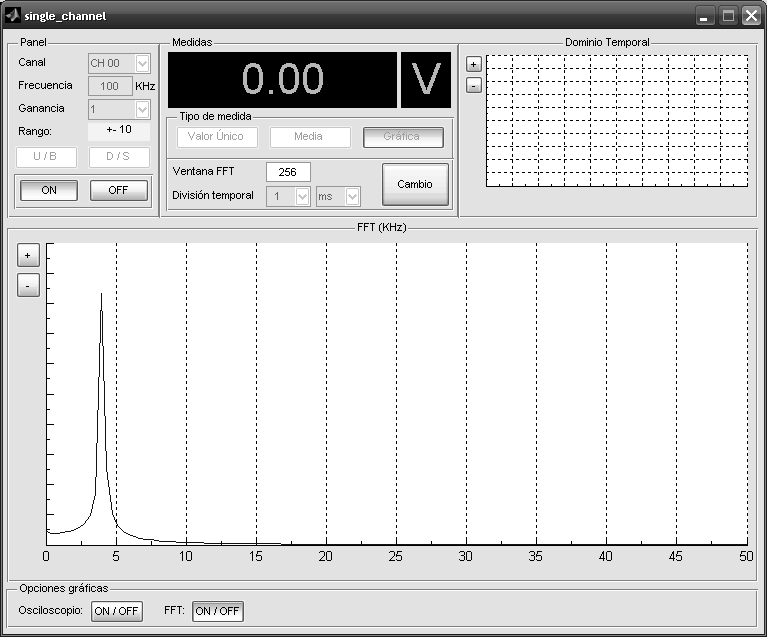
\includegraphics{gis-pfc-ch4-03.png}
    \end{center}
    \caption[Representación de la señal inhabilitada]{Representación de la
    señal inhabilitada.}
    \label{fig:signal-disabled}
\end{figure}

\begin{figure}[p]
    \begin{center}
	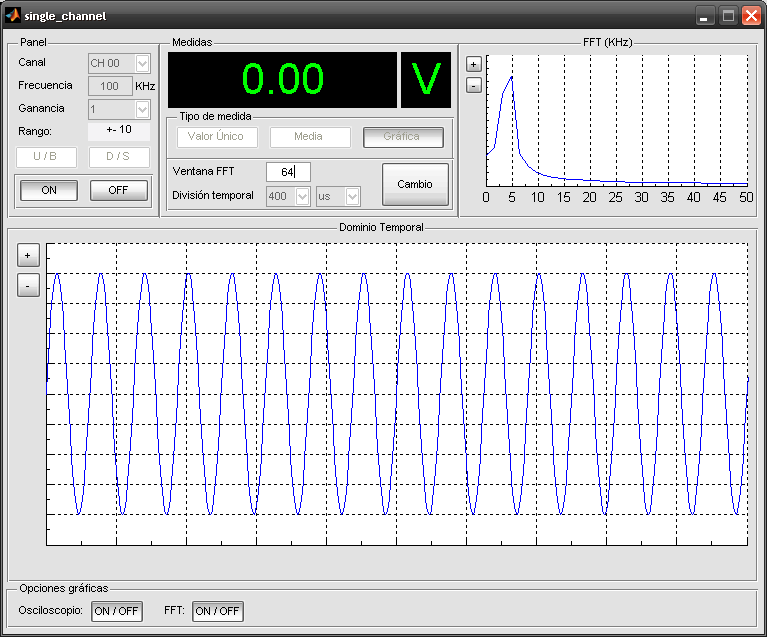
\includegraphics{gis-pfc-ch4-04.png}
    \end{center}
    \caption[Selección de otra escala temporal]{Se representa la señal
    empleando una escala temporal distinta (duración del fragmento
    representado por defecto de 1 ms, duración seleccionada $0.4$ ms).}
    \label{fig:scaled}
\end{figure}

\begin{figure}[p]
    \begin{center}
	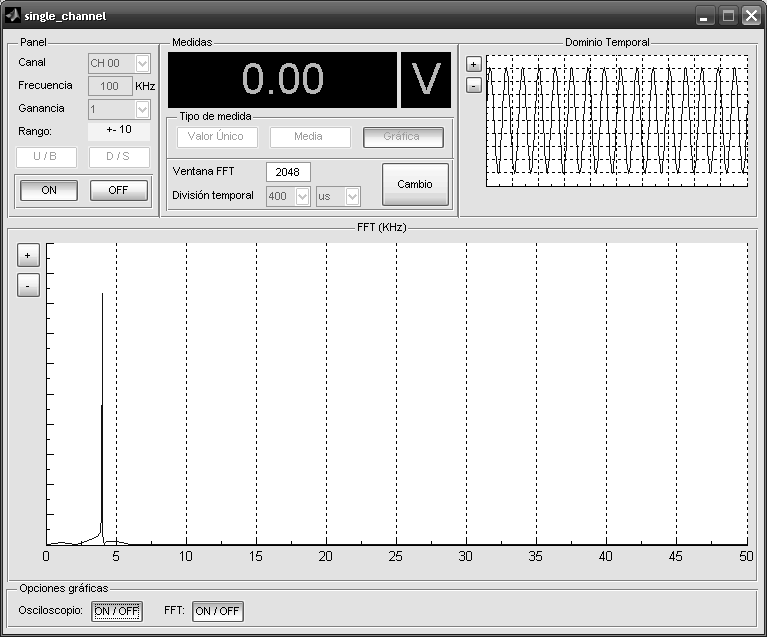
\includegraphics{gis-pfc-ch4-05.png}
    \end{center}
    \caption[Selección de un número de puntos distinto para la realización
    de la \sig{fft}]{Selección de un número de puntos distinto para la
    realización de la \sig{fft}.}
    \label{fig:point-number}
\end{figure}


\section{Conclusiones y futuras líneas de trabajo}

Los resultados observados en apartados anteriores certifican que se ha
logrado desarrollar satisfactoriamente un sistema de medida con las
siguientes prestaciones:

\begin{itemize}
    \item Seguimiento del valor numérico instantáneo de la señal.
    \item Cálculo de la media aritmética cada 250 ms.
    \item Representación gráfica continua o disparada de la señal.
    \item Simultáneamente, representación gráfica del espectro en
	frecuencias de la señal (\sig{fft}).
\end{itemize}

Este sistema de medida presenta, no obstante, las siguientes limitaciones
conocidas:

\begin{itemize}
    \item Inherentes a los componentes del sistema:
	\begin{itemize}
	    \item La frecuencia de las señales que pueden representarse
		correctamente está limitada a 25 kHz.
	    \item El modo continuo de representación (adecuado para
		representar señales de frecuencia inferior a 5 Hz) no
		funciona apropiadamente en equipos sin aceleración gráfica.
	    \item La caja de conexiones induce la aparición de señal en
		puertos situados en la misma fila que el puerto utilizado.
	\end{itemize}
    \item Inherentes al código fuente de la aplicación:
	\begin{itemize}
	    \item La aplicación carece de las funciones de autoajuste y
		disparo automático.
	    \item La aplicación no muestra medidas automáticas de los
		parámetros de la señal.
	    \item Los controles para ajustar la escala temporal, el número
		de puntos para el cálculo de la \sig{fft} y la escala de
		amplitud pueden mejorarse.
	    \item La aplicación carece de cursores para evaluar
		gráficamente los parámetros de la señal.
	    \item No es posible seleccionar la frecuencia con la que se
		calcula la media aritmética de los datos obtenidos.
	\end{itemize}
\end{itemize}

En el futuro sería recomendable actualizar el equipo que conforma el
sistema de medida, especialmente la tarjeta de adquisición, para obtener
unas mejores prestaciones. Además es posible mejorar la aplicación
incorporando nuevas funcionalidades a las que ya están disponibles.


\subsection{Subsistema para la interacción con el medio
físico}\label{subsec:transducerconclusions}

El sistema de medida digital obtenido como resultado del proceso de diseño
y desarrollo que ocupa esta primera parte del proyecto se pone a prueba al
realizar una serie de ensayos ultrasónicos preliminares que pretenden
evaluar la capacidad del sistema para encontrar resultados válidos. Estos
ensayos se realizan en el laboratorio a partir de muestras extraídas de
palmeras muertas (listones y tablones de madera de palmera). Los resultados
arrojados por las pruebas demuestran que el pulso ultrasónico que emite el
actuador no es capaz de atravesar los tablones de 20 cm de espesor
utilizados en el experimento. Se llega por tanto a la conclusión de que los
transductores de gama baja utilizados para la confección del subsistema
para la interacción con el medio físico, a pesar de ser apropiados para
aplicaciones como un detector de proximidad, no reúnen las condiciones
necesarias para ser utilizados en un \sig{endus}.

Además, un estudio posterior realizado durante el desarrollo de este
documento ha revelado el importante papel que adquieren los circuitos de
acondicionamiento en los ensayos no destructivos por ultrasonidos. Por todo
ello se recomienda la renovación de los transductores, por unos de mayor
potencia, y una vez renovados éstos, la realización de los circuitos
acondicionadores apropiados para extraer el máximo partido a los nuevos
transductores.
